\documentclass[11pt,a4paper]{report}
\usepackage[spanish,es-nodecimaldot]{babel}	% Utilizar español
\usepackage[utf8]{inputenc}					% Caracteres UTF-8
\usepackage{graphicx}						% Imagenes
\usepackage[hidelinks]{hyperref}			% Poner enlaces sin marcarlos en rojo
\usepackage{fancyhdr}						% Modificar encabezados y pies de pagina
\usepackage{float}							% Insertar figuras
\usepackage[textwidth=390pt]{geometry}		% Anchura de la pagina
\usepackage[nottoc]{tocbibind}				% Referencias (no incluir num pagina indice en Indice)
\usepackage{enumitem}						% Permitir enumerate con distintos simbolos
\usepackage[T1]{fontenc}					% Usar textsc en sections
\usepackage{amsmath}						% Símbolos matemáticos

% Comando para poner el nombre de la asignatura
\newcommand{\asignatura}{Simulación de sistemas}
\newcommand{\autor}{Adrián Acosa Sánchez}
\newcommand{\titulo}{Ejercicio de Montecarlo}
\newcommand{\subtitulo}{Problema de la lechería}
\newcommand{\rama}{Computación y Sistemas Inteligentes}

% Configuracion de encabezados y pies de pagina
\pagestyle{fancy}
\lhead{\autor{}}
\rhead{\asignatura{}}
\lfoot{Grado en Ingeniería Informática}
\cfoot{}
\rfoot{\thepage}
\renewcommand{\headrulewidth}{0.4pt}		% Linea cabeza de pagina
\renewcommand{\footrulewidth}{0.4pt}		% Linea pie de pagina

\usepackage{graphicx}
\begin{document}
\pagenumbering{gobble}

% Pagina de titulo
\begin{titlepage}

\begin{minipage}{\textwidth}

\centering

%
\includegraphics[scale=0.5]{img/ugr.png}\\

\includegraphics[scale=0.3]{img/logo_ugr.jpg}\\[1cm]

\textsc{\Large \asignatura{}\\[0.2cm]}
\textsc{GRADO EN INGENIERÍA INFORMÁTICA}\\[1cm]

\noindent\rule[-1ex]{\textwidth}{1pt}\\[1.5ex]
\textsc{{\Huge \titulo\\[0.5ex]}}
\textsc{{\Large \subtitulo\\}}
\noindent\rule[-1ex]{\textwidth}{2pt}\\[3.5ex]

\end{minipage}

%\vspace{0.5cm}
\vspace{0.7cm}

\begin{minipage}{\textwidth}

\centering

\textbf{Autor}\\ {\autor{}}\\[2.5ex]
\textbf{Rama}\\ {\rama}\\[2.5ex]
\vspace{0.3cm}


\includegraphics[scale=0.3]{img/etsiit.jpeg}

\vspace{0.7cm}
\textsc{Escuela Técnica Superior de Ingenierías Informática y de Telecomunicación}\\
\vspace{1cm}
\textsc{Curso 2022-2023}
\end{minipage}
\end{titlepage}

\pagenumbering{arabic}
\tableofcontents
\thispagestyle{empty}				% No usar estilo en la pagina de indice

\newpage

\setlength{\parskip}{1em}

\chapter{Problema de Montecarlo}
\newpage

\section{Descripción del problema}

Se quiere hacer un estudio de una lechería que produce 1000 litros de leche al día y que envasa en latas de 10 litros cada una, por lo que producen 100 latas al día. El almacen que tiene la lechería sólamente puede almacenar 200 latas, y el precio de venta varía en función de cuántas latas haya al final del día anterior:

\begin{itemize}
	\item{Más de 125 latas, al día siguiente la lata se vende a 1 euro.}
	\item{Menos de 75 latas, al día siguiente la lata se vende a 2 euros.}
	\item{En cualquier otro caso, al día siguiente se vende a 1.50 euros.}
\end{itemize}

\begin{tabular}{cccc}
	\hline
	1 euro & 1.50 euros & 2 euros & Demanda\\
	\hline
	0.1 & 0.15 & 0.30 & 50\\
	0.2 & 0.30 & 0.40 & 90\\
	0.3 & 0.35 & 0.20 & 130\\
	0.4 & 0.20 & 0.10 & 170\\
	\hline
\end{tabular}

Los días en los que el stock inicial más la producción supera la capacidad del almacen, se dona la cantidad excedente a instituciones de la caridad.

Una vez tenemos todos los datos del problema, es hora de montar el montecarlo.

\section{Planteamiento de la simulación}

Todo lo explicado en este apartado se puede apreciar mejor si se ve el código al mismo tiempo.

Para llevar a cabo el modelo, lo primero que tenemos que hacer es lo que hacemos siempre con un modelo de Montecarlo que es crear nuestra función que nos genere un uniforme entre 0 y 1. 

Una vez tenemos nuestro generador de números uniformes ya podremos crear nuestro generador de demandas. Para el generador de demandas hemos usado el método de tablas de búsqueda, en la que tenemos que tener en cuenta que las probabilidades de las demandas varían en función del precio que haya ese día. Por lo tanto los parámetros que usaremos para el generador de demandas serán los distintos valores de demanda indicados (que las crearemos en el main ya que siempre tendrán los mismos valores) y las probabilidades que tienen cada una de las demandas (que también le pasaremos como parámetro al ser variables en función del stock, cosa que controlamos en el bucle de la simulación comprobando el tamaño que tiene el almacen al final del día).

Ya tenemos los generadores de datos necesarios para poder realizar la simulación. Ahora vamos con la simulación en sí. Para ello lo que tenemos que hacer es inicializar las variables que usaremos para calcular las medias fuera del bucle de la simulación. También, como he comentado en el párrafo anterior, aquí es donde se inicializa la tabla que aparece en la descripción del problema en tres arrays distintos: uno para las demandas y otros tres para las distintas probabilidades en función del stock.

El siguiente paso es realizar un bucle que ejecute varios meses para ser lo más precisos posibles. Para ello lo que tendremos que hacer es pedirle al usuario un número de veces que ejecutar el bucle y así ver cómo es el transcurso de todos los meses. Yo el número de meses que he usado para simular el sistema ha sido 10000, ya que ejecutando varias veces con 10000 meses los valores obtenidos no varían tanto como con 100 o 1000 meses.

Lo que vamos a hacer para simular el problema es que en cada día vamos a sumar 100 latas al almacen y comprobar si podemos almacenarlo o no, y en función de esta condición acumularlas en el almacen o donarlas, respectivamente. Tras esto, generamos la demanda en función del stock del día anterior (empezando con el almacen con 20 latas y por tanto con el precio a 2 euros) y vamos comprobando si podemos satisfacer o no la demanda. Si no podemos satisfacer la demanda, acumulamos las latas que no hemos podido vender en su contador correspondiente. Por último, lo que hacemos es ajustar la tabla de probabilidades según el número de latas que resten en el almacen para generar la demanda en el siguiente día.

\section{Simulación}
El resultado que obtenemos con 10000 meses es el siguiente:
\begin{itemize}
	\item{Media de latas donadas: 90.928 latas}
	\item{Media de latas no vendidas: 122.941 latas}
	\item{Media de días sin espacio suficiente en el almacen: 4.2528 días}
	\item{Media de días sin satisfacer la demanda: 3.7388 días}
\end{itemize}

\begin{figure}[H]
\begin{tabular}{ll}
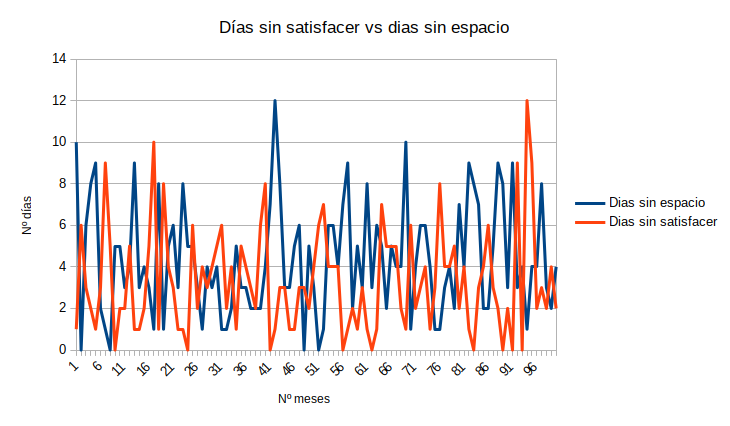
\includegraphics[scale=0.25]{img/dias_sin_espacio_satisfacer.png}
&
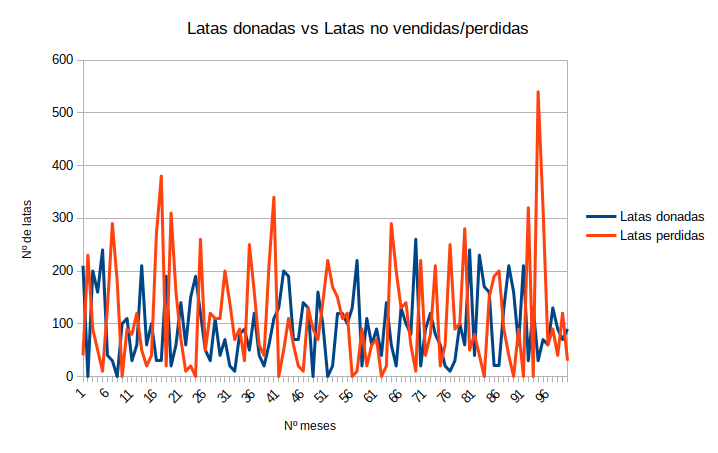
\includegraphics[scale=0.25]{img/no_vendidas_donadas.png}
\end{tabular}
\caption{Comparaciones entre las distintas situaciones posibles}
\end{figure}

\section{Conclusiones y posibles mejoras de la lechería}

Viendo los resultados del modelo, lo más lógico es que se amplíe el tamaño del almacen para no se done tanto y no se pierdan tantas posibles ventas. Pero si solo aumentamos el tamaño del almacen y dejamos la producción al mismo nivel lo que va a pasar es que dejaremos de donar pero seguiremos en algunos casos sin poder satisfacer la demanda como es el caso de esta ejecución: 

\begin{figure}[htp]
\centering
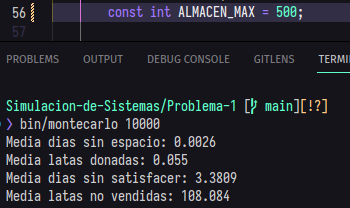
\includegraphics[scale=0.4]{img/aumento_almacen.png}
\caption{Ejecución aumentando el tamaño del almacén a 500 latas}
\label{}
\end{figure}

Por tanto, habría que aumentar un poco la producción para que se de la situación ideal en la que ni se donen latas por exceso, ni falten latas por defecto.

\end{document}

